\graphicspath{{contextProbImages/}}
\chapter{Contexte et problématique}

\section{Contexte : L'essor des agents conversationnels}

\subsection{L'intelligence artificielle}

Ce qui est artificiel a généralement une connotation négative car on le perçoit comme moins bien que l’objet réel. Mais dans la réalité, l’objet artificiel est souvent au-dessus car plus performant. Si on prend le cas d’une fleur artificielle, la fleur ne requiert pas d’eau ni soleil et aura la même utilité qui est de décorer.
\vspace{1em}

L’intelligence artificielle est comme la fleur, elle n’est pas naturelle car elle est la création de l’homme. Il faut comprendre le sens d’intelligence et le définir \cite{ref2}.
\vspace{1em}

	Une définition de R. Sternberg, psychologue et professeur de psychologie cognitive américain : “ L'intelligence est la capacité cognitive d'un individu pour apprendre de son expérience, bien raisonner, se rappeler des informations importantes et faire face aux demandes de la vie quotidienne.”
\vspace{1em}

	Le but de l’intelligence artificielle est de créer des programmes ou systèmes qui ont une pensée similaire à celle d’un humain. Il faut faire une distinction entre la pensée et l’intelligence car la pensée est la faculté de raisonner, analyser, évaluer et proposer des idées alors que les êtres capables de penser ne sont pas forcément intelligents.
	\vspace{1em}

	Il y a des degrés d’intelligence parmi les humains, les humains et aussi les IA. C’est en $1950$ qu’Alan Turing a établi une méthode pour évaluer celle d’une IA.
\vspace{1em}

	Aujourd’hui l’intelligence artificielle est basée sur des algorithmes de règles ainsi que sur de l’apprentissage sur le temps avec des données pour l’entraîner. Les bots ne répondent pas simplement aux questions des utilisateurs mais les guident pour avoir la question la plus précise et donc répondre le mieux aux besoins \cite{ref3}.
	\vspace{1em}


\begin{figure}[H]
	\centering
		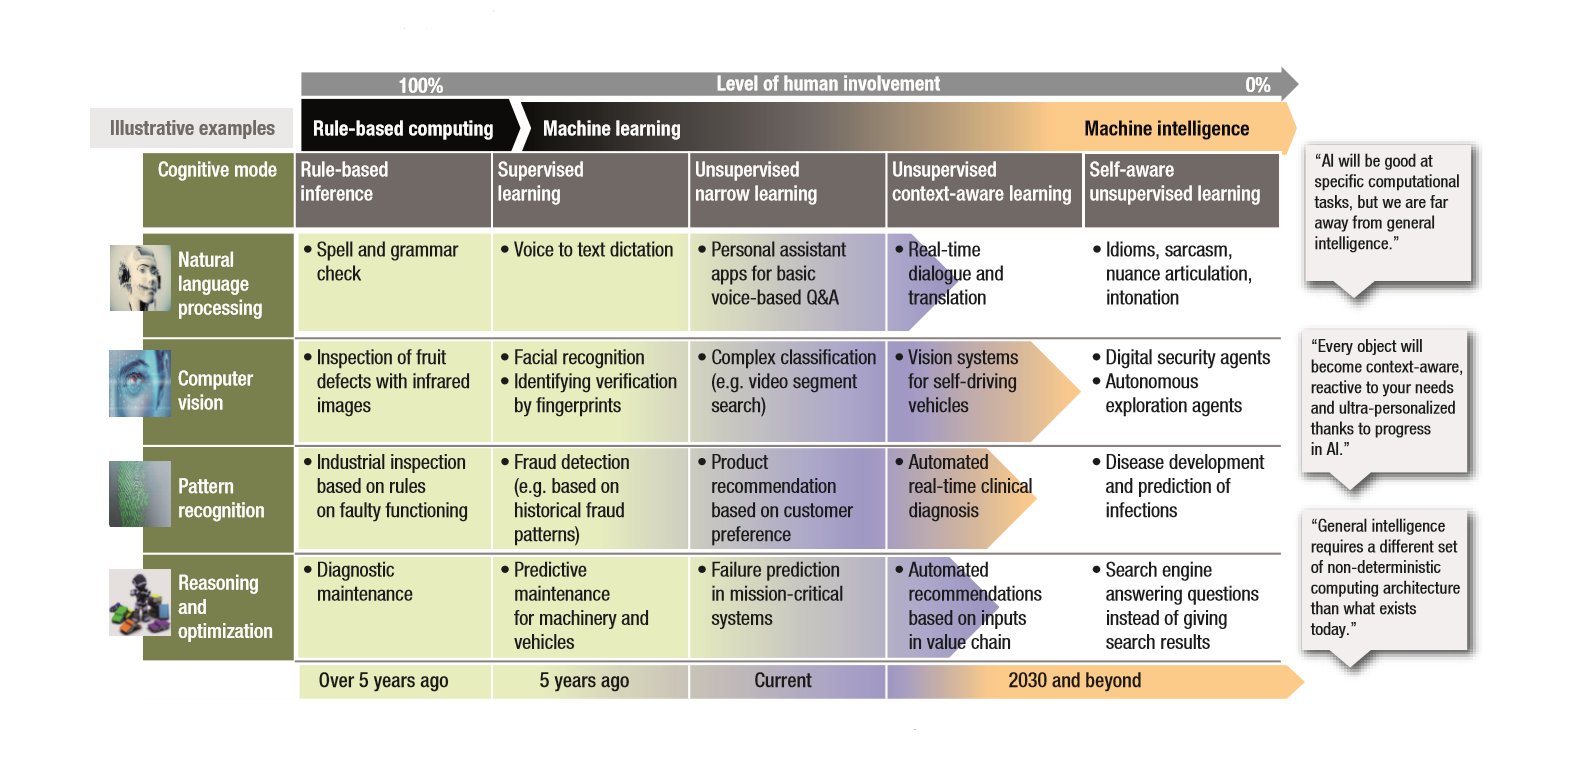
\includegraphics[width = \textwidth]{AI.png}
	\caption{Développement de l'IA et ses états}
	\label{fig:AI evolution}
\end{figure}



Dans le domaine du dialogue, l’IA est liée au natural language processing que l’on abordera dans la partie concept. On remarque, en se penchant sur l’évolution (figure \ref{fig:AI evolution}), qu’on commence à avoir du dialogue temps-réel et il y a davantage de langues compréhensibles avec un passage de l’une à l’autre par la traduction. On cherche à atteindre un dialogue où l’on peut comprendre un sens caché d’un dialogue comme le sarcasme, l’humour ou encore l’intonation pour les dialogues oraux.
\vspace{1em}

	Ce progrès est dû en grande partie aux avancées de la puissance de calcul et les algorithmes d’apprentissage mais aussi au coût des ordinateurs et des espaces de stockages qui a fortement baissé.
\vspace{1em}

	Pour le moment, l’intelligence artificielle est vue comme un service pour beaucoup d’entreprises. En effet, elle aurait pour but de réduire les coûts de production, dynamiser des processus, offrir des produits et des services hyper-personnalisés basés sur les préférences des clients.“Messaging apps will introduce a paradigm shift for marketers… new conversational interfaces will drive deeper relationships between consumers and brands.” Forrester.
\vspace{1em}


	Pour les dialogues, on est à l’ère des assistants personnels que l’on nomme agents conversationnels qui fournissent un service en dialoguant avec un utilisateur. Microsoft, Google, Facebook, IBM et Amazon commencent à investir dans ces agents pour utiliser leurs propres services.
“’Conversational AI-first’ will supersede "cloud-first, mobile-first" as the most important, high-level imperative for the next $10$ years, AI will be a $5$B business by $2020$.”Gartner.
\vspace{1em}



\subsection{L'agent conversationnel}

Un agent conversationnel/chatbot est un programme perçu par les utilisateurs comme une personne artificielle, un animal ou autre qui tient des conversations avec les humains. Cela peut être  une conversation écrite, orale ou non verbale. \cite{ref4}
\vspace{1em}

	Les chatbots sont un phénomène : 
	\vspace{1em}
	
« Au cours des derniers mois, les chatbots ont investi le devant de la scène tech. Tous les grands noms du secteur ont apporté leur pierre à l’édifice, que ce soit au travers d’une nouvelle interface conversationnelle ou bien en développant une intelligence artificielle. Google a la volonté de prendre le leadership dans le domaine de l’intelligence artificielle, les annonces dans le domaine sont quasi-quotidiennes » \cite{ref5}.
\vspace{1em}

	On reparle des bots car facebook ouvre messenger aux bots en avril 2016 \cite{ref6}.
Mark Zuckerberf explique qu’avec l’IA et le natural language processing combiné à de personnes réelles, les gens parleront aux bots sur messenger comme s’ils parlaient avec leurs amis.
\vspace{1em}

	Les chatbots sont une nouvelle manière d’interagir avec des services existants, une expérience utilisateur novatrice qui laisse entrevoir de nombreuses opportunités.
	\vspace{1em}
	
	De plus, il y a une demande très forte. Cela s’explique notamment par le fait que, depuis fin $2015$, l’utilisation des applications de messagerie a surpassé celle des réseaux sociaux et l’utilisation des sms \cite{ref4}. Cette présence massive et croissante des utilisateurs sur ces interfaces conversationnelles est donc un nouvel « Eldorado » pour les marques. 
	\vspace{1em}
	
	Cependant, les applications de messagerie ne sont pas la seule explication de cette démocratisation. L’intelligence artificielle est au cœur de la plupart des services conversationnels et au cours des précédentes années, ce domaine de l’informatique a considérablement progressé, entraînant avec lui les chatbots.

\subsection{Cas d'utilisation}

Dans les années $2010$, on a les premiers systèmes de dialogue homme-machine grand public sur divers sites Internet, robots de compagnie, téléphones portables, agendas électroniques, systèmes de géolocalisation et autres assistants personnels.
\vspace{1em}

	Au niveau des systèmes grand public, on est loin  d’un dialogue en langage naturel. Par exemple, les systèmes de géolocalisation et les téléphones portables en sont encore à la détection de mots-clés : noms de ville, noms de destinataires. Loin de la compréhension de « je veux aller à Grenoble en contournant Lyon et en évitant l’autoroute entre Saint-Etienne et Lyon »
\vspace{1em}	


	\begin{figure}[H]
	\centering
		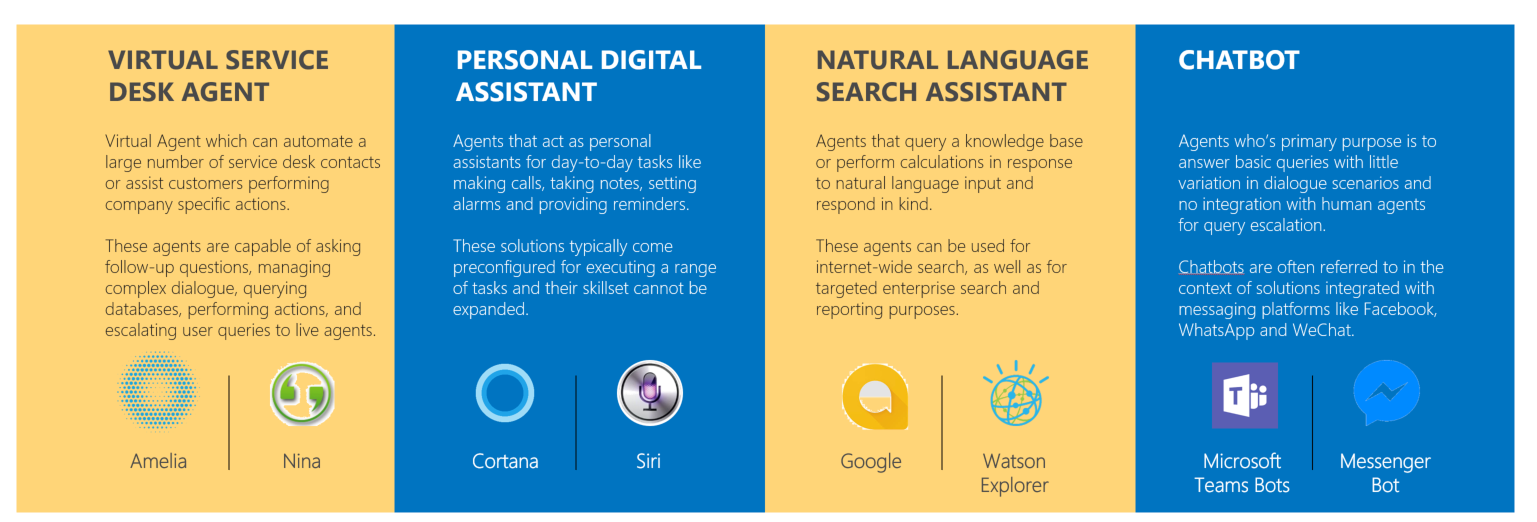
\includegraphics[width =\textwidth]{agents.png}
	\caption{Différents agents conversationnels actuels}
	\label{fig:Agents conversationnels}
\end{figure}

Il y a des chatbots internes aux entreprises, par exemple pour organiser un meeting, regarder qui est disponible, proposer un horaire disponible pour tous les participants, puis la réservation d’une salle. Le chatbot ne fait que consulter les calendriers et proposer des choix, le seul dialogue est celui pour proposer des participants, choisir une date et un lieu. Aucune autre information ne peut être demandée.
\vspace{1em}	

	Et des chatbots offrent un service payant comme Pizza Hut sur facebook messenger. Il faut prendre contact avec le compte officiel Pizza Hut (être son ami). Quand le bot est sollicité, il présente trois options : passer commande, découvrir les promotions et « autre » (service client avec de vraies personnes). En passant commande, il est possible d’afficher les dernières commandes passées ou d’afficher le menu. Le paiement peut s’effectuer en ligne ou sur place. Quand on choisit de passer une commande, on entre dans un formulaire où le bot pose les questions et l’utilisateur répond. L’utilisateur ne pourra pas poser des questions et il sera bloqué.
	\vspace{1em}	
	
D’autres chatbots : 
\begin{itemize}
	\item Bot météo : donne la météo quand on lui demande
	\item Bot actualités : on lui demande si des choses intéressantes se passent dans l’actualité
	\item Bot de vie : on lui dit nos problèmes et il essaye de trouver une solution
	\item Bot ami : En Chine, il y a un bot appelé Xiaoice créé par Microsoft, avec 20 millions qui lui ont parlé.
\end{itemize}


\section{Problématique}

	Il y a deux types de chatbots : un simple avec des règles et l’autre plus intelligent avec du machine learning.
	\vspace{1em}	
	
	Le chatbot basé sur des règles est très limité. Il va répondre à des commandes spécifiques. Si ce qu’on lui dit ne fait pas partie de ces commandes alors il ne comprend pas.
	\vspace{1em}	
	
	Alors que le chatbot basé sur le machine learning a une IA. Il comprend en partie le language naturel et n’a pas juste des commandes. De plus, le machine learning lui permet d’apprendre en discutant avec les utilisateurs.
	\vspace{1em}	
	
	Comme nous l’avons vu plus haut, les cas d’utilisation sont pour l’instant basiques. En effet, le problème majeur du bot est de comprendre l’utilisateur. Le bot ne peut pas comprendre le langage naturel sauf si on lui a fait apprendre certaines phrases types. C’est pour ça que des formulaires ou encore une sélection d’actions sont mis en place dans un dialogue avec un bot pour avoir un dialogue à domaine fermé. (figure \ref{fig:Complexité d'un bot})
	\vspace{1em}	
	
	\begin{figure}[H]
	\centering
		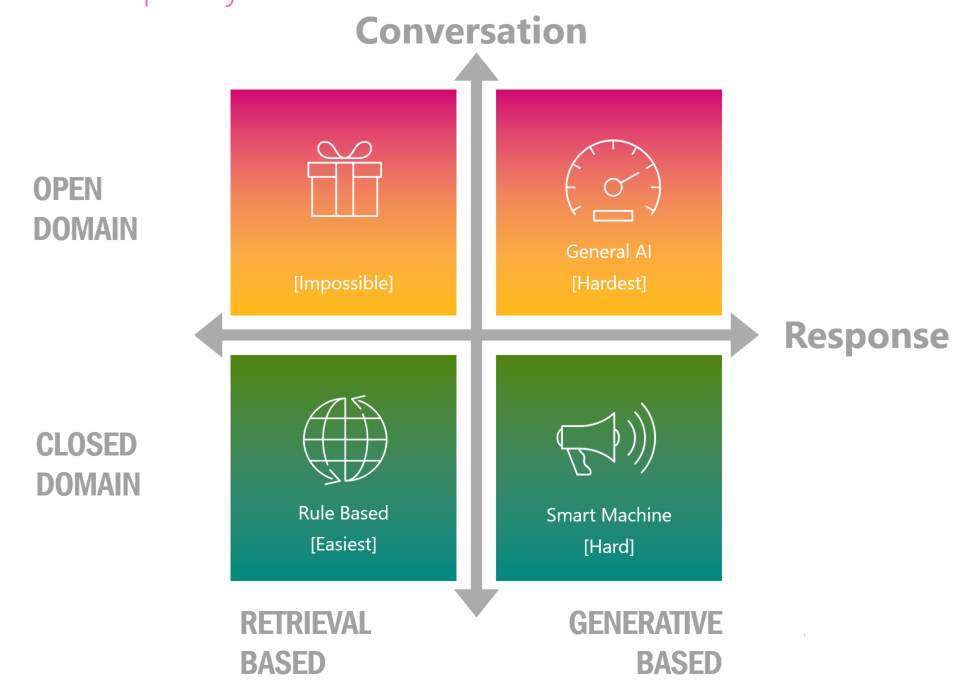
\includegraphics[width =\textwidth]{complexe.png}
	\caption{Complexité d'un bot}
	\label{fig:Complexité d'un bot}
\end{figure}

Pour créer un bot, on doit réfléchir à la façon dont on veut le faire interagir avec l’utilisateur. Pour cela, on va se concentrer sur le dialogue homme-machine, avec la phase compréhension du langage humain qui correspondra au natural language understanding et on réfléchira aussi à la façon d’extraire les données pour être ensuite analysées  et former une réponse qui sera la phase natural language generation.
\vspace{1em}

	Dans ce mémoire, on se posera la question suivante : en quoi comprendre le dialogue homme-machine de façon théorique permet-il de créer un bot ?
	\vspace{1em}
	
	Les littératures scientifiques sur les IA et plus récemment sur les chatbots ont fait émerger différentes solutions dont  nous parlerons dans ce mémoire.